\chapter{Introduction}
\label{ch:intro}

\section{Motivation}

The rapid evolution of \textit{Cooperative, Connected and Automated Mobility (CCAM)} is transforming modern transportation systems.
CCAM technologies enable vehicles to communicate with each other and with infrastructure, promising safer, more efficient, and more sustainable mobility~\cite{ertrac2022ccam}.
As intelligent transportation systems become increasingly reliant on machine learning for critical functions such as route optimization, traffic prediction, and safety-critical decision-making, the accuracy and reliability of these models directly impact both operational efficiency and public safety.
Recent trends in CCAM emphasize the need for real-time adaptability and continuous model refinement as urban environments become more complex and data-driven~\cite{abdi2021travel}.

However, achieving reliable predictions in such dynamic settings presents significant challenges.
One key use case is \textit{Estimated Time of Arrival (ETA)} prediction for vehicles, a core service in smart mobility that influences traffic management, logistics, and traveler information~\cite{abdi2021travel}.
Many current mobility systems do not continuously recalibrate their prediction models as new data arrives~\cite{arifi2024eta}.

\section{Problem Statement}

Urban mobility environments are highly dynamic and \textit{non-stationary}, meaning that the statistical properties of traffic data change over time.
Machine learning models trained on static historical data often assume a fixed data distribution, an assumption that rarely holds in real city conditions~\cite{gama2014survey}.
When deployed in a dynamic urban setting, a model's performance can gradually degrade as driving patterns shift due to \textit{concept drift}, the evolution of the underlying data relationships over time~\cite{lu2018learning}.
This drift is triggered by many factors: for example, road network changes (e.g., construction) can alter traffic flow patterns significantly~\cite{maheshwari2025survey}.
Even routine variations like weather and seasonal demand swings can lead to abrupt or gradual shifts in vehicle speeds and congestion levels.
A model that performs well on dry, low-traffic days may become less accurate during heavy rain or rush-hour peaks if those conditions were not part of its training distribution~\cite{baier2020error}.
The challenge is that static ML models struggle to maintain accuracy in the face of non-stationarity, as their predictive power deteriorates over time unless the models continually adapt to the evolving urban mobility data~\cite{gama2014survey}.

While concept drift detection and adaptation techniques have been well-studied in the literature~\cite{lu2018learning, greco2025drift}, what remains largely unaddressed is the lack of a \textit{holistic, integrated platform} specifically tailored for CCAM environments.
Existing solutions are often fragmented or confined to laboratory settings, lacking the integration of critical components needed for systematic drift management in distributed mobility scenarios.
Current tools may address individual aspects, such as drift detection or model retraining, but they rarely incorporate traffic simulation, continuous monitoring, and adaptive retraining into one seamless, automated loop~\cite{xin2024lit, modesto2025self}.

This gap motivates the creation of a continuous machine learning platform for mobility: one that integrates traffic simulation to test "what-if" scenarios, live performance dashboards to observe errors as they evolve, drift detection algorithms to raise alerts when model performance degrades, and an automated retraining pipeline to deploy updated models.
By monitoring performance through time rather than just offline metrics and triggering adaptation with minimal human intervention, we aim to ensure that mobility prediction models remain accurate and robust despite the ever-changing urban environment, ultimately supporting the safety and reliability requirements of CCAM applications.

\begin{figure}[ht]
    \centering
    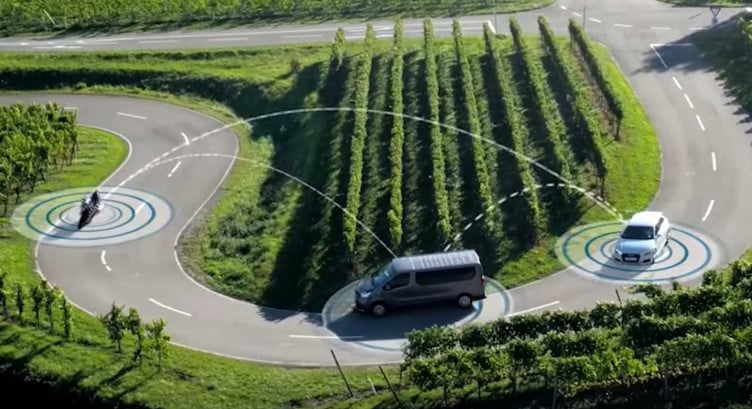
\includegraphics[width=0.7\textwidth]{figures/ccam.png}
    \caption{Cooperative, Connected and Automated Mobility (CCAM).}
    \label{fig:ccam}
\end{figure}

\section{Thesis Goal}

The objective of this thesis is to design, implement, and evaluate a microservice-based platform for \textit{continuous machine learning} in urban mobility applications.
In essence, the goal is to create a \textit{drift-aware ML platform} that supports end-to-end monitoring and adaptation of predictive models in a city traffic context.

To achieve this, we first establish a reproducible experimental foundation by developing a synthetic dataset generation pipeline using the SUMO traffic simulator~\cite{krajzewicz2012recent}.
This addresses a critical gap: the lack of standardized, publicly available drift benchmarks in urban mobility research.
By leveraging SUMO's microscopic traffic simulation capabilities, we can generate controlled scenarios that include both stable conditions and deliberate drift events, such as weather-induced traffic changes, providing labeled data for model training and realistic drift testing.
This synthetic approach ensures reproducibility, allows for systematic experimentation with different drift patterns, and enables validation of the platform's drift detection and adaptation mechanisms in a controlled yet realistic environment.

Building upon this data foundation, the platform will be built using a modular microservice architecture to ensure scalability and flexibility, where each component (orchestration, model serving, drift detection, etc.) operates as an independent service.
Crucially, the platform is intended to be model-agnostic and domain-specific: it can host any machine learning model for mobility prediction tasks, but this thesis will demonstrate and evaluate it primarily through the lens of an Estimated Time of Arrival (ETA) prediction use case.
We focus on ETA because of its importance in CCAM scenarios, helping vehicles and travelers coordinate effectively, and because it provides a tangible benchmark to test how well the platform handles concept drift.
Upon detecting drift, it will automatically trigger model adaptation, i.e. retraining and model swapping, to self-correct the predictions.

Although ETA is the main case study, the system is designed to accommodate additional models. For example, external predictive modules for Fuel Consumption~\cite{angelis2025fuel} and Number of Stops~\cite{tzelepis2025stops} will be integrated to showcase that multiple concurrent mobility models can coexist and benefit from the shared drift-aware infrastructure.
By the end of this thesis, we aim to show that such a platform can be realized and that it effectively maintains model performance over time in a realistic urban traffic setting.

\section{Contributions}

This thesis makes several contributions to the state of the art in continuous machine learning for mobility:

\begin{itemize}
    \item \textbf{Synthetic Dataset Pipeline:} We developed a reproducible, modular data pipeline that generates training and evaluation datasets using synthetic traffic data from Simulation of Urban MObility (SUMO)~\cite{krajzewicz2012recent}.
        Focusing on a case study of central Athens, the pipeline takes an open-source city road network and creates realistic traffic scenarios (vehicles, routes, events) to produce rich labeled data.
        This approach ensures that experiments are repeatable and tunable, meaning that the pipeline can be re-run for any city region or traffic pattern by adjusting parameters, thus addressing the shortage of standard drift benchmarks in urban mobility.

    \item \textbf{ETA Prediction Model under Drift:} We designed a feature-engineered ETA prediction model using gradient-boosted decision trees (LightGBM)~\cite{ke2017lightgbm}.
        The model is trained on the above dataset to estimate travel times for vehicles, and we introduce domain-specific features to improve accuracy.
        More importantly, the model's performance is evaluated under highly-realistic simulation-based drift scenarios, e.g., a sudden shift from normal traffic to heavy rain conditions that reduce vehicle speeds.
        This allowed us to study how concept drift affects ETA prediction accuracy, and to validate that our model, and platform, can detect and respond to these changes.

    \item \textbf{Time-Lapse Drift Simulation:} We conducted a time-lapse simulation experiment to rigorously assess drift detection and adaptation in an end-to-end fashion.
        In this setup, the SUMO simulator replays an extended sequence where an initial period of stable conditions is followed by a clear drift event, in this case a transition from dry weather to a storm causing slower traffic.
        The platform's drift detectors monitor the real-time prediction error and successfully detect the concept drift when the environment changes.
        We then measure how the system's automatic adaptation, triggering model retraining with new data from the rainy period, helps recover the model's performance.
        This exploration provides a realistic validation of the platform's ability to observe, detect, and mitigate drift in a controlled yet lifelike scenario.

    \item \textbf{Drift-Aware Platform Implementation:} We present the design and implementation of a platform for continuous machine learning in mobility, which is a key practical contribution of this work.
        The platform includes components for simulation replay that feed historical or synthetic data through the model as if in real time, live dashboarding of model performance metrics, so that users can visualize concept drift as it happens, pluggable drift detection algorithms with calibration tools to set detection thresholds and minimize false alarms, and an automatic retraining and deployment pipeline, which seamlessly replaces the old model with an updated one when drift is confirmed.
        The entire system is built with modern software frameworks, such as containerized microservices, REST APIs for model serving, and event-driven triggers for retraining, to ensure it can be deployed in real operational environments.
        By open-sourcing the platform and detailing its architecture, we enable other researchers and practitioners to reproduce our approach and extend it to their own cooperative and automated mobility applications.

\end{itemize}

\section{Thesis Structure}

The remainder of this thesis is structured as follows:

\begin{itemize}
    \item \textbf{Chapter 2: Background} - Introduces the foundational concepts and tools underlying our work.
        We review machine learning basics relevant to continuous model updating, the notion of concept drift, such as types of drift and common detection methods, the SUMO traffic simulator and its functionalities for creating mobility scenarios, and the platform technologies, like microservices, Docker, and APIs, used to build our solution.

    \item \textbf{Chapter 3: Related Work} - Surveys existing literature and systems in areas pertinent to our thesis.
        We cover drift detection tools and frameworks, examples being streaming ML libraries and MLOps solutions for model monitoring, and review prior research on ETA prediction models in classic and intelligent transportation.
        Finally, we discuss how our approach compares to and innovates upon the current state of the art.

    \item \textbf{Chapter 4: Dataset and Modeling} - Details our methodology for creating the dataset and developing the ETA prediction model.
        We describe the data generation process using SUMO for the Athens case study, including how traffic demand patterns and drift scenarios, in this case weather changes, are configured.
        We then present the ETA model development, including feature engineering, hyperparameter tuning, model selection, and the overall training procedure and the set up of the experiments.

    \item \textbf{Chapter 5: Platform Architecture} - Provides a comprehensive overview of the drift-aware platform's design.
        We enumerate the microservices and their roles, explain how the system ingests data, either from simulation or future extensions to real streams, how drift detection algorithms are integrated, and how the platform orchestrates retraining and deployment of models.
        Implementation details of key components, such as the real-time dashboard, are given to illustrate how the system works in practice.

    \item \textbf{Chapter 6: Results} - Presents the results of our evaluation.
        We report the baseline performance of the ETA model under static conditions and then analyze its behavior under induced drift.
        We demonstrate the effectiveness of drift detection and quantify the gains from automatic adaptation.
        The results validate the platform's ability to maintain model accuracy over time.

    \item \textbf{Chapter 7: Conclusions} - Summarizes the contributions and findings of the thesis.
        We reflect on the success of the continuous machine learning approach for CCAM applications and any limitations observed.
        Finally, we outline future research directions, such as improvements to platform scaling and monitoring, or integrating the system with real-time data streams.

\end{itemize}
